%%%%%%%%%%%%%%%%%% Changelog %%%%%%%%%%%%%%%%%% 


%% 01 April 2008	Henrik Frisk	mail@henrikfrisk.com

%% 30 March 2008	Henrik Frisk	mail@henrikfrisk.com
%%% Melecn code: MELECON-0247

%% Section II.C:
%% 28 March 2008	Henrik Frisk	mail@henrikfrisk.com

%% Section I: 
%% Moved footnote 1 to be associated with Integra rather than EC:
%% "...Birmingham Conservatoire in the UK^1..."

%% Footnote 6:
%% Typo in URL: "http://..."

%% Section II.C:
%% "globally unique symbolic name" shouldn't this be something like
%% "for the context globally..."? Is it an error to have to modules
%% with the same symbolic name? As long as they have §different
%% namespaces (/mypiece/sinus1 and /myotherpiece/sinus1) it's
%% perfectly OK isnt't it? The UID however must be unique. NO CHANGE
%% MADE YET!!!

%% Section II.C, para 2:
%% Typo. Extra first character ('>').

%% Section III.A:
%% Updated all XML examples to reflect the current Schema. As this is much more compact all attributes fitted, hence the parenthesis "(please note that only the \emph{freq}-attribute is included)" was removed.

%% Section V:
%% Space before footnoe 9 removed. Changed all but the first occurence of "Postgresl" to "Postgres" as stated in footnote 9.

%% Section VI.B: 
%% Typo in last sentence: "a! ccessed"

%% Section VI.C:
%% Added two sentences at the end.

%% Section VII, first para:
%% changed reference to sourceforge to name with URL in footnote for consistency.


%%%%%%%%%%%%%%%%%% / Changelog %%%%%%%%%%%%%%%%%% 

\documentclass[10pt,journal,final]{IEEEtran}
\usepackage{graphicx}
\usepackage{url}

\newcommand\T{\rule{0pt}{2.6ex}}
\newcommand\TT{\rule{0pt}{3.6ex}}
\newcommand\B{\rule[-1.2ex]{0pt}{0pt}}
\newcommand\BB{\rule[-2.2ex]{0pt}{0pt}}
% correct bad hyphenation here
\hyphenation{op-tical net-works semi-conduc-tor}

\begin{document}
\pagestyle{empty} 

\title{Sustainability of `live electronic' music in the Integra project}

%%\author{James Bullock\and Henrik Frisk\and and Lamberto Coccioli \thanks{Supported by...}}

\author{\thanks{This work is part financed by the European Commission through the 2005 call of the Culture 2000 programme [ref 2005-849] and by the Integra project members.}
  James Bullock\thanks{J.\,Bullock is with the Music Technology Department at Birmingham Conservatoire, Birmingham City University, Birmingham, B3 3HG, UK (e-mail: james.bullock@bcu.ac.uk)}%
  \and, Henrik A. Frisk\thanks{H.\,A.\,Frisk is with the Performance, Composition and Church Music Department at Malm\"{o} Academy of Music, Lund University, Box 8203, 20041 Malm\"{o}, Sweden (e-mail: henrik.frisk@mhm.lu.se)}
  \and and Lamberto Coccioli\thanks{L.\,Coccioli is  with the Music Technology Department at Birmingham Conservatoire, Birmingham City University, Birmingham, B3 3HG, UK (e-mail: lamberto.coccioli@bcu.ac.uk)}}

%\IEEEspecialpapernotice{(Invited Paper)}

% make the title area
\maketitle

\thispagestyle{empty}

\begin{abstract}
In this paper we describe a new XML file format and a database schema designed for the storage of performance data and meta-data relating to live electronic music. We briefly describe the architecture of the Integra environment, and give examples of the hierarchical modelling of Integra classes. The separation of module definition, module instance data and module implementation data is presented as one of the key components of the Integra system. The libIntegra library is proposed as a means for supporting the file formats in target applications.
\end{abstract}

\begin{keywords}
Documentation, Multimedia databases, Multimedia systems, Music, Programming environments, Software portability
\end{keywords}

\section{Introduction}\label{sec:introduction}

Integra, ``A European Composition and Performance Environment for Sharing Live Music Technologies", is a 3-year project led by Birmingham Conservatoire in the UK\footnote{\url{http://www.integralive.org}} and supported by the Culture 2000 programme of the European Commission. One aspect of Integra is to develop a new software environment to facilitate composing and performing in the context of interactive and live electronic music. In general, the project attempts to address the problems of persistent storage, portability and standardised intercommunication between different software (and hardware) systems for electronic music. It is a priority that all data relating to supported musical works, including scores, electronic parts, information about different versions and renderings of these works, biographical data, etc., should be stored on a web-accessible database, and that this data should be transferable to a variety of usable target applications.

Integra started as a way of standardising the construction of modules, and providing a generalised OSC namespace within the Max/MSP environment. As such it has some similarities with the Jamoma\cite{Place:01}\footnote{\url{http://www.jamoma.org/}} and Jade projects\footnote{\url{http://www.electrotap.com/jade}}. However, it now differs substantially from either of these in that it has a strong emphasis on software independence, and persistent storage. Two other projects that aim to tackle problems that are similar to those which Integra attempts to address are Faust \cite{Orlarey:01}\cite{Orlarey:02}\footnote{\url{http://faust.grame.fr}} and NASPRO\footnote{\url{http://sourceforge.net/projects/naspro/}}. Furthermore, Integra's repertoire migration programme \cite{BullockCoccioli:01} is closely related to documentation and technology migration initiatives such as the PD Repertory Project\cite{Puckette:01}, Mustica\cite{Bachimont:01}, and the CASPAR Project\footnote{\url{http://www.casparpreserves.eu/}}, though the scope of the latter is much wider than that of Integra.

\section{Integra modules}\label{sec:modules}

The basis of the Integra library is the concept of the Integra module. Integra modules encapsulate a specific piece of message or signal processing functionality. A module could perform a simple task like generating a sine wave, or a complex task like emulating a specific synthesiser. In this section, we will outline how Integra modules and module collections are constructed.

\subsection{Module construction}\label{subsec:module_construction}

The minimum requirement for an Integra module is that it must have an interface definition. In addition, it may also have an implementation and module instance data. Of these, only the implementation is software specific.

\subsubsection{Module definition}\label{subsubsec:module_definition}

An Integra module definition is data that defines what attributes a module has, and what the characteristics of those attributes are. An Integra attribute is a symbolic name with which a value can be associated. The module definition doesn't store the actual values of attributes, instead it stores data about the attributes such as their names, descriptions, supported data types, maxima and minima, and default values. Typical module definition data is shown in Table \ref{tab:module_definition}.

\begin{table}[b]
\caption{Integra Oscillator interface definition}
\begin{center}
\begin{tabular}{|l|l|}
\hline
\textbf{Field} & \textbf{Value} \\
\hline
Name  & Oscillator \\
\hline
Parent  & Module \\
\hline
Attributes & freq, phase \\
\hline
Attribute Unit Codes & 1, 2 \\
\hline
Attribute Minima & 0, 0 \\
\hline
Attribute Maxima & inf, 6.2831853071795862 \\
\hline
Attribute Defaults & 440, 0 \\
\hline
\end{tabular} 
\end{center}
\label{tab:module_definition}
\end{table}

The parent field is used to show an inheritance relation. All Integra module definitions could be thought of as class definitions, the members of which are all abstract (lack implementation), or interface definitions. The interface of a given class can inherit the interface of any other class, and supplement this with additional members. This definition hierarchy is the basis of the Integra database (see section \ref{sec:database}). 

\subsubsection{Module namespace}\label{subsubsec:module_namespace}

A module's namespace is derived from its definition. The namespace enables the values of attributes to be set, and module methods to be called  by using a symbolic naming scheme.  From the user's perspective, this will usually manifest itself as an OSC address space. The OSC address space for a sinus module is shown in Table \ref{tab:module_namespace}. The sinus class inherits the oscillator class interface, which in turn inherits the module class interface, so all of these must be reflected in the module's namespace, and in turn must be represented in the implementation.

\begin{table}[h]
\caption{Integra Sinus module namespace}
\begin{center}
\begin{tabular}{|p{17em}|p{8em}|} %%{|p{20em}|p{20em}|}
\hline
\textbf{OSC address} & \textbf{Purpose} \\
\hline
\begin{minipage}[0pt]{10em}
\small {
\begin{verbatim}/oscillator/freq <value>\end{verbatim}}\end{minipage}  & \small{Set the value of the `freq' attribute} \\
\hline
\begin{minipage}[0pt]{10em}
\small{
\begin{verbatim}/oscillator/phase <value>\end{verbatim}}\end{minipage}  & \small{Set the value of the `phase' attribute} \\
\hline
\begin{minipage}[0pt]{10em}
\small{
\begin{verbatim}/module/active <value>
\end{verbatim}} \end{minipage} & \small{Set whether or not the module is active} \\
\hline
\end{tabular} 
\end{center}
\label{tab:module_namespace}
\end{table}

\subsubsection{Module implementation}\label{subsubsec:module_implementation}

The module implementation is the only software-specific data stored by Integra. It consists of a fragment of computer code, in one or more files, which when run or loaded by a particular piece of software will perform a specific audio or message processing task. In order that module implementations can be used by libIntegra, an implementation protocol must be devised for each software target. Integra currently provides implementation protocols for Max/MSP and Pure Data (Pd) along with a growing selection of example module implementations and implementation templates. In practice, the implementation files are Max and PD `abstractions' that provide a number of compulsory methods, and conform to the implementation protocol. A typical module implementation is shown in Figure {\ref{fig:sinus}}. 

\begin{figure}[b]
\centerline{\framebox{
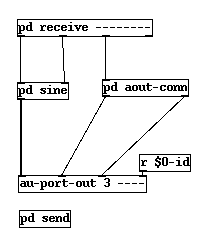
\includegraphics[width=14em]{img/integra-sinus}}}
\caption{An Integra sine wave oscillator implemented in PD}
\label{fig:sinus}
\end{figure}

A SuperCollider class to perform the same task, might look as follows:
{\small
\begin{verbatim}
Sinus : Oscillator {
    init{
     var freq, outPorts, server;
     freq = 440;
     outPorts = [1];
     actions = actions.add(
       {|val| this.server.sendMsg(
         ``/n_set'', nodeid, \freq, val)});
     nodeid = Synth(\Sinus, 
       [\freq, freq, \outport0, outPorts[0]]
       ).nodeID;
     super.init;
    }
}
\end{verbatim}}
This implementation is very different from the PD sinus, not only because it is implemented in a different module host (i.e. SuperCollider), but also because it employs inheritance to provide much of its functionality. In SuperCollider we can use inheritance at the level of implementation to mirror the interface inheritance used in the Integra database, and conceptually between abstract Integra classes. The PD sinus must implement all of the interfaces inherited by the sinus class and its parents, right to the top of the class tree. The SuperCollider sinus only needs to implement the interface that is unique to it, implementations of inherited interfaces are inherited from the parent class: Oscillator. 

In the short term, the Integra project seeks to provide protocol specifications for constructing module implementations in a range of different software environments. A longer term goal is to explore ways in which the process of constructing module implementations may be automated.

\subsubsection{Module instance data}\label{subsubsec:module_instance_data}

Module instance data consists of the run-time state of all of its variable parameters. This data is stored in memory by the Integra library whilst a module is in use, and can be written to an XML file on demand. In addition, for persistent storage, the same data can be stored in the Integra database in the module's instance table. Currently only one saved state can be associated with each module instance.

\subsection{Module collections}\label{subsec:module_collections}

An Integra collection consists of one or more Integra module instances. A collection can also contain other collections. These contained collections encapsulate the functionality of a number of connected Integra modules into a single entity and can be addressed and connected as if they were normal module instances. The facility is provided for collections to optionally expose the input and output parameters of the modules they contain. For example, the collection `mySinus' might contain a Sinus module, which has the attributes Frequency and Phase, but the collection might only expose the Frequency attribute to the containing collection, whilst setting the Phase to some arbitrary constant value.

\subsection{Module ports}\label{subsec:module_ports}

Modules and collections are connected up to each other using Integra ports. Each port corresponds to an audio or messaging address, which has both a symbolic name and a numeric identifier (port ID). Port symbolic names correspond to a module's attribute names (e.g. `freq'), and port numbers are derived implicitly from the index of the port in the module's attribute list. 
In addition to its port number, each module has unique symbolic name
(e.g. `sinus1') within its scope,\footnote{There are currently three possible containing scopes for
a module instance: `collection', `encapsulated collection' and `aggregator'.} and an implicitly determined, globally
unique numeric identifier (UID).
The Integra library can be used to address any module port using either their fully-qualified symbolic name (e.g. `/sinus1/oscillator/freq'), or using a combination of their UID and port ID. It is an important part of the Integra module construction protocol that port ordering is always consistent. Otherwise a module implementation's port numbering will not correspond to the numbering expected by the Integra library.

From the perspective of the Integra library, database, and XML schema,
there is no distinction between audio and control rate ports. This
distinction is only made in the implementation. There is also no
conceptual distinction between input ports and output ports, a port is
just an address that can receive data and connect to other addresses.
This is illustrated in figure \ref{fig:sinus} where the `pd receive'
object corresponds to ports one to four, which in turn correspond to
oscillator frequency, oscillator phase, the audio output and the module `active' setting. In this example, ports one, two and four will set the attributes of the sine oscillator when sent a numeric value, and report their current value to any connected ports when sent an empty message.

\subsection{Connections}\label{subsec:connections}

For each module or collection, the Integra library stores a list of ports that each output port of a given module is connected to. One-to-many, many-to-one or many-to-many connections can easily be established. However, it is important to note that providing this functionality makes it a requirement for the software hosting the modules to support these routings. Table \ref{tab:lib_namespace} lists some of the commands used to intantiate and connect/disconnect modules in the instance host.

\begin{table*}
\caption{Instance host OSC scheme}
\begin{center}
\begin{tabular}{|p{27em}|p{21.5em}|}
\hline
\textbf{Command} \T \B & \textbf{Purpose} \\
\hline
\begin{minipage}[0pt]{20em}
\small {
\begin{verbatim}/load <module-name>\end{verbatim}} \end{minipage} \T & \small{Instantiate a module in a given target} \\
\hline
\begin{minipage}[0pt]{20em}
  \small {
\begin{verbatim}
/remove <module id>
\end{verbatim} 
}
 \end{minipage} \T
& \small{Remove a module instance} \\
\hline
\begin{minipage}[0pt]{20em}
\small {
\begin{verbatim}
/connect<module id> <port number> 
     <module id> <port number> 
\end{verbatim} 
}
 \end{minipage} \TT
& \small{Connect two ports} \BB \\
\hline
\begin{minipage}[0pt]{20em}
\small {
\begin{verbatim}
/disconnect <module id> <port number> 
         <module id> <port number> 
\end{verbatim}
}
 \end{minipage} \TT
& \small{Disconnect two ports} \BB \\
\hline
\begin{minipage}[0pt]{20em}
\small {
\begin{verbatim}/send <module id> <port number> <value> 
\end{verbatim} 
}
 \end{minipage} \T
& \small{Send a value to a port} \\
\hline
\begin{minipage}[0pt]{20em}
\small {
\begin{verbatim}
/direct <module id> <state> \end{verbatim}
} \end{minipage} \T
& \small{Toggle direct message passing for a module instance} \BB \\ 
\hline
\end{tabular} 
\end{center}
\label{tab:lib_namespace}
\end{table*}

\section{IXD (Integra eXtensible Data)}\label{sec:ixd}

In order to store modules, module collections, and performance data in a software-neutral manner, a bespoke Integra file format was developed. XML was chosen as the basis for this since it is relatively human-readable, can be transformed for a variety of output targets, and has a number of excellent tools for parsing, reading and writing. The library currently uses the libxml2\footnote{\url{http://xmlsoft.org/}} library to provide much of its XML processing functionality.

Rather than keeping all data needed to store an Integra collection in a single file we make use of the XML Linking language (XLink\footnote{\url{http://www.w3.org/TR/xlink/}}) to link in relevant resources. This makes for more efficient parsing and helps to keep file sizes small.

\subsection{Integra module definition}\label{subsect:integra_class_definition}

Perhaps the most important part of the IXD specification is the module definition file. It is the XML representation of an Integra module (see \ref{subsubsec:module_definition}). These files are created and updated through the database interface and stored locally for offline access in a gzipped archive. Each file contains the class and module definitions of one unique module and a link to the parent class from which it inherits properties:

{\small
\begin{verbatim}
<Class>
 <ClassDefinition>
   <name>Sinus</name>
   <parent ...
        xlink:href="Oscillator.xml">
        Oscillator
   </parent>
    ...
 </ClassDefinition>
 <ModuleDefinition>
    ...
 </ModuleDefinition>
</Class
\end{verbatim}
}
All documents that are part of the Integra documentation system must have a class definition - it represents the super class of the Integra class hierarchy and it defines those attributes shared by all kinds of data - performance data, biographical data, etc. (see section \ref{subsubsec:module_definition}). The module definition is specific to the notion of \emph{modules} as defined in section \ref{sec:modules}.

A part of the body of the module definition IXD file containing the definition shown in Table \ref{tab:module_definition}, would contain the following construct:

{\small
\begin{verbatim}
<attribute id="md.0">
  <unit>ntgHz</unit>
  <description>The value in Hz (0 - INF).
  </description>
  <minimum>0.0</minimum>
  <maximum>INF</maximum>
  <default>440</default>
</attribute>
<attribute id="md.1">
  <unit>ntgRadians</unit>
  <description>The value in Radians 
               (0 - 2PI).</description>
  <minimum>0.0</minimum>
  <maximum>6.2831853071795862</maximum>
  <default>0</default>
</attribute>
<attribute id="md.1">
  <unit>ntgBoolean</unit>
  <description>Is the module active?
  </description>
  <default>true</default>
</attribute>
 ...
\end{verbatim}
}

Each module and each of its attributes may also hold a documentation reference. This allows the implementing host for this module to make a call to the instance host to bring up on-line documentation, for this attribute or for the module itself. The link points to a file included in the local archive of module descriptions.
{\small
\begin{verbatim}
<attribute id="cd.0">
  <name>freq</name>
  <documentation title="Documentation of the 
                        frequency attribute." 
                 href="FrequencyDoc.xml" 
                 ... />
</attribute>
\end{verbatim}
}

\subsection{Integra collection definition}\label{subsect:integra_collection_definition}

Once a module is defined and stored in an IXD file it may be instantiated. Instances of classes of modules along with their inter-connections are stored in a collection file which is the Integra equivalent of a PD or Max/MSP `patch'.

In a collection file each module instance is represented by a locator that points to the definition of the class to which the instance belongs. Connections between ports are represented by \emph{arcs} between resources in the module definition file pointed to by the locator. Finally, it also holds references to performance data files.

% \subsection{The IXD file format  summary}
\section{libIntegra}\label{subsec:db_lib}

libIntegra\cite{bullockfrisk:01} is a cross-platform shared library, mostly written in ISO C89 compliant C, and packaged using the GNU autotools tool chain. It consists of a common API, and a number of optional components.

libIntegra provides application developers with all of the functionality required to read, write and validate Integra-compliant XML. It can also be used for module instantiation in a target application via an application specific bridge. The library has a set of SWIG-generated Python bindings, which enable the same XML serialisation code to be used on a remote database server and in a local application. For further details regarding the library's design see \cite{bullockfrisk:01}.

\section{Database}\label{sec:database}

For persistent storage of module data and other data relating to musical works we have designed and configured an on-line database. The database comprises a Postgresql\footnote{Postgres hereafter.} back-end, and a web-based UI written in Python. Postgres was chosen because of its reliability, maturity and close-coupling with the data-structures to be stored. Because Postgres is an object-relational database management system (ORDMS), we were able to utilise the facility to create inheritance relations between tables, mirroring inheritance between module classes. We also make extensive use of Postgres' array type.

In the Integra database, the module definitions are stored in one table, with references to data in a number of supplementary look-up tables. For example, the module definition shown in Table \ref{tab:module_definition} would be stored in a single row in the Module Definitions table. Data in fields such as `Attribute Unit Codes' are stored as integers that are used as indices to a look-up table. This is done to ensure data consistency, efficiency of storage and fast look-up.

The `Attribute Units' look-up table might look as shown in Table \ref{tab:lookup_table}.

\begin{table} 
\caption{Typical look-up table}
\begin{center}
\begin{tabular}{|l|l|}
\hline
\textbf{Field} \T \B & \textbf{Value} \\
\hline
1 & Hertz \T \\
\hline
2 & Radians \T \\
\hline
\end{tabular} 
\end{center}
\label{tab:lookup_table}
\end{table}

\subsection{Database UI}\label{subsec:db_ui}
Users may add new, or edit existing module definitions via a web-based interface. The interface also provides mechanisms for uploading and downloading module definitions, and collections.
Once a module definition has been added to the definitions table, the database schema is extended through the addition of a corresponding table to hold the new module's instance data. When a module definition is added to the database, the module's parent is specified, and only attributes that differ from those provided by its parent are added. An inheritance relation is then created between the new module's instance table, and the parent module's instance table. This means that all of the parent module's attributes then become available to instances of the child module.

\section{Use case examples}\label{sec:use_case}
Since the Integra XML file format, database schema and associated protocols are currently under development, it has not seemed prudent to develop `finished' migrations of existing works using the system, or to construct new works that rely on the system in performance. However a range of works have been transferred to new technology as part of the Integra project, and these serve as an essential support for the continuing development of the Integra framework. The Integra library and protocols also form the basis of a number of other systems. Some of these will outlined briefly in the following sections.

\subsection{Integra GUI}\label{sec:integra_gui}
The Integra GUI is a central aspect of the Integra project, and forms one of the primary reasons for the libIntegra development. The purpose of the GUI is to provide a powerful but simple interface for musicians to work with live electronics and develop their ideas. So far a prototype GUI has been developed, and this has served as useful testbed for establishing the utility of the libIntegra library as providing a foundation for usable software.

\subsection{{\it Madonna of Winter and Spring}}\label{subsec:madonna}
This was one of the first works to be ported for Integra. It initially formed part of the `Harvey Project' (now the FreeX7 project\footnote{\url{http://www.conservatoire.bcu.ac.uk/freex7}}), which predates the Integra project. The migration of {\it Madonna of Winter of Spring} is described in detail in \cite{BullockCoccioli:01}, but to summarise, the most significant technical problems posed by the work centre on the emulation of a Yamaha TX816 and Yamaha DX1, both of which are based on the Yamaha DX7 synthesis model. The work was ported to the Pd environment using a bespoke Pd-based DSSI plugin host, and the open source Hexter DX7 emulation plugin. Subsequently, the TX816, DX1 and DX7 synthesisers have been made into Integra-compliant modules, instantiable using libIntegra, and addressable using an Integra DX namespace. The DX7 and TX816 namespaces are available via the Integra wiki\footnote{\url{http://wiki.integralive.org/modules:dx7}}, and the respective modules can be accessed through the Integra subversion repository\footnote{\url{http://svn.integralive.org}}.

\subsection{Other projects}\label{subsec:other_projects}
The Integra library has been used in the PhD work of two of the current authors. It forms the `backend' for the Sonar 2D\footnote{\url{http://postlude.co.uk/Software/Sonar2D}} application by Jamie Bullock, providing DSP module instantiation, management and persistent storage. It is also being used by Henrik Frisk in the documentation, presentation and implementation of a number of pieces included in his artistic PhD thesis. These projects have served as an excellent `real world' test-bed for the library's functionality and experiences are fed back into the development.

\section{Project status}\label{sec:status}

Integra is currently hosted on Sourceforge\footnote{\url{http://sourceforge.net}}. We have a small but active developer community which is growing slowly as the project progresses. The Integra environment is the core goal of the development strand of the Integra project, and seeks to provide a complete, expandable and sustainable solution to compose and perform music with interactive live electronics.
libIntegra and a bespoke GUI for the Integra environment are currently in pre-alpha development.
 
\subsection{Future work}\label{subsec:future}

One of current priorities is to populate the Integra database with a large number of module definitions and implementations. However, we would like to keep the amount of implementation-specific data we store to an absolute minimum. The first step in this has been to separate out the module definition, namespace (derived from the definition), instance data, and implementation. We would now like to explore ways of storing the data encoded by the implementation in a software-neutral manner. One way to do this might be to create a set of implementation primitives, and then create more complex modules from these using Integra collections as an encapsulation mechanism. Another possibility would be to create a simple Integra scripting language that could be used in addition to module encapsulation, or alongside a DSP description language such as Faust \cite{Orlarey:02} 

\section{Conclusion}\label{sec:conclusion}

We have outlined a new XML-based file format for storing data relating to live electronic music. The format is environment-neutral, and is closely coupled with an in-memory representation used by the libIntegra library and a persistent representation that uses an object-relational database. In addition we have suggested the libIntegra library as the de-facto means for accessing and manipulating Integra modules, and interfacing with specific audio software environments. The next stage in our work will entail a phase of alpha and beta testing, both internally and with our end users. The aim of the Integra project is to improve the usability of software for working with live electronics, and to provide a robust mechanism for the sustainability of existing repertoire and new musical works. libIntegra and its associated file formats should ultimately provide a foundation for this.


% \section{References}
% \label{sec:references}

\begin{thebibliography}{citations}

\bibitem{Orlarey:01} Orlarey, Y. and Fober, D. and Letz, S.
''Syntactical and semantical aspects of FaustSoft Computing''
{\it Soft Computing - A Fusion of Foundations, Methodologies and Applications}, vol. 8, no. 9, 2004

\bibitem{Orlarey:02} Orlarey, Y. and Fober, D. and Letz, S.
''An Algebra for Block Diagram Languages''
{\it Proceedings of the International Computer Music Conference}, ICMA, USA, 2002.

\bibitem{Place:01} Place, T. and Lossius, T.
''Jamoma: A Modular Standard for Structuring Patches in Max''
{\it Proceedings of the International Computer Music Conference}, ICMA, USA, 2006.

\bibitem{Puckette:01} Puckette, M.
''New Public-Domain Realizations of Standard Pieces for Instruments and
Live Electronics''
{\it Proceedings of the International Computer Music Conference}, ICMA, USA, 2006.

\bibitem{Bachimont:01} Bachimont, B. and Blanchette, J.-F. and Gerzso, A. and Swetland, A. and Lescurieux, O. and Morizet-Mahoudeaux, P. and Donin, N. and Teasley, J.
''Preserving interactive digital music: a report on the MUSTICA research initiative''
{\it Web Delivering of Music, 2003.} 2003 WEDELMUSIC. Proceedings. Third International Conference on Web Delivering of Music.

\bibitem{bullockfrisk:01} Bullock, J. and Frisk, H.
''libIntegra: a system for software-independent multimedia module description and storage''
{\it Proceedings of the International Computer Music Conference}, ICMA, Sweden, 2007.

\bibitem{BullockCoccioli:01} Bullock, J. and Coccioli L.
"Modernising musical works involving Yamaha DX-based synthesis: a case study"
{\it Organised Sound 11(3)}, Cambridge University Press, UK, 2006

\end{thebibliography}
\newpage
\section{Biographies}
\label{sec:biographies}
\flushbottom
\begin{biography}[{
\includegraphics[width=1in,height=1.25in,clip,keepaspectratio]{./img/jamie}}]
Jamie Bullock (b.1977) is a specialist in musical composition and
performance with interactive technology. He studied composition with
Francois Evans and Andrew Deakin at Middlesex University and with Jonty
Harrison at the University of Birmingham. He is also a self-taught
computer programmer.

In 2004, he was awarded a research bursary by Birmingham Conservatoire,
where he currently teaches on the BSc and BMus programmes. In 2006 he
was appointed as Research Assistant and he is currently engaged in a
number of national and international research collaborations including
the European-funded Integra project.

Jamie enjoys hill-walking, cooking and eating, and has a life-long
commitment to developing the right software for the job.
\end{biography}
\begin{biography}[{
\includegraphics[width=1in,height=1.25in,clip,keepaspectratio]{./img/frisk}}]
Henrik Frisk, born in Antibes, France on June 11, 1969, and studied in Copenhagen, New York and Malm\"{o}. He is currently doing his final year of his PhD studies at The Malm\"{o} Academy of Music, Lund University. 

He is an active performer of improvised and contemporary music and composer of chamber and computer music. After having pursued a career in jazz in the nineties with performances at the Bell Atlantic Jazz Festival, NYC and Montreux Jazz Festival, Switzerland, he is now spending most of his time composing and playing contemporary music with a recent interest in sound installation and sound art. He has performed in Belarus, Canada, Chech Republic, China, Cuba, Denmark, Finland, France, Germany, Iceland, India, Mexico, Norway, Poland, Sweden, Switzerland and the United States. Henrik Frisk is also a renowned teacher, having taught at The Rhythmic Conservatory in Copenhagen and was the head of department for Jazz and Improvised Music at Malmö Academy of Music. As a visiting lecturer he has given lectures at several schools and universities, mainly in Scandinavia.
\end{biography}
\begin{biography}[{
\includegraphics[width=1in,height=1.25in,clip,keepaspectratio]{./img/lamberto}}]
Lamberto Coccioli is Head of Music Technology at Birmingham Conservatoire. After reading architecture and art history
in Rome he studied composition with Azio Corghi in Milan and attended master classes with Pierre Boulez, Elliott Carter
and George Benjamin. Of lasting influence were a series of journeys to remote areas of Colombia to record music and
sounds of traditional Indian and mestizo communities.

In 1994 he began an extended collaboration with Luciano Berio, and two years later he joined Tempo Reale, the research
centre for new technologies applied to music founded by Berio in Florence. He worked there as a composer, teacher,
performer and artistic coordinator.

Since arriving in Birmingham in 2000 he has been developing a wide range of activities and resources to integrate new
technologies within the Conservatoire's programmes. He created the Conservatoire’s Centre for Composition and
Performance with Technology and supervised the renovation of the Conservatoire’s Recital Hall, a unique space for the
performance of multimedia and live electronics works. He's currently managing Integra, a 3-year EU-funded project to
promote and disseminate music with live electronics.
\end{biography}
\end{document}

